\ylDisplay{Äpardus plokiga} % Ülesande nimi
{Tundmatu autor} % Autor
{lõppvoor} % Voor
{2014} % Aasta
{P 10} % Ülesande nr.
{3} % Raskustase
{
% Teema: Mehaanika

\ifStatement
\begin{center}
	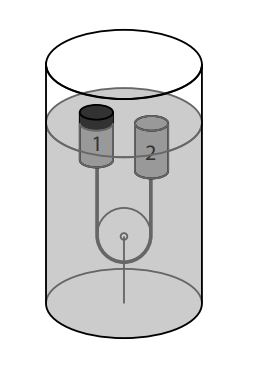
\includegraphics[width=0.5\linewidth]{2014-v3p-10-yl.PNG}
\end{center}
Silindrilises anumas põhjapindalaga $S$ on vesi tihedusega $\rho$. Anuma põhjas on plokk ja üle hõõrdevabalt pöörleva plokiratta on tõmmatud nöör. Nööri otste külge on kinnitatud kaks veest väiksema tihedusega keha. Plokk takistab nende kehade veepinnale kerkimist (vt joonis). Kummagi keha ruumala on $V$ . Ühe keha tihedus on $\rho 1$ ja teise keha tihedus $ \rho 2$, kusjuures $\rho1 < \rho2 < \rho$. Plokinöör on nii pikk, et kumbki kehadest ei puuduta plokki ning nii lühike, et üks keha on tõmmatud üleni vee alla. Kui palju muutub anumas oleva vee tase kui plokinöör katkeb ja mõlemad kehad kerkivad vee pinnale?
\fi

\ifHint
Alustuseks hinda anuma põhja poolt süsteemile "vesi pluss kehad" mõjuva jõu muutust. 
\fi

\ifSolution
Arvutame anuma põhja poolt süsteemile "vesi pluss kehad" mõjuva jõu muutuse
\begin{center}
$\triangle F = -2T = S \rho g \triangle h$,
\end{center}
kus $T$ on nööri pinge. Tõepoolest, nimetatud jõud tasakaalustab kõikide ülejäänud jõudude resultandi, milleks on raskusjõudude summa (ei muutu), pluss nööri poolt mõjuv jõud. Et nööri pinge hoiab teist keha vee all, siis $T = (\rho - \rho_2)gV$, millest
\begin{center}
$\triangle h = -\frac{2(\rho - \rho_2) V}{S \rho}$.
\end{center}
\fi
}